\documentclass[tikz,border=8pt]{standalone}
\usepackage{amsmath}
\usetikzlibrary{arrows.meta,calc}

\definecolor{blockblue}{RGB}{74,144,217}
\definecolor{sumgreen}{RGB}{92,184,92}
\definecolor{taporange}{RGB}{240,173,78}
\definecolor{linegray}{RGB}{51,51,51}

\tikzset{
  signal/.style={-{Stealth[length=3mm,width=2mm]}, line width=1.2pt, draw=linegray},
  block/.style={rectangle, draw=blockblue, line width=1.2pt, fill=none, align=center, minimum width=1.125cm, minimum height=0.75cm, font=\footnotesize\bfseries},
  smallblock/.style={block, minimum width=1.0cm, minimum height=0.75cm},
  auxblock/.style={block, minimum width=1.7cm, minimum height=0.9cm},
  plant/.style={block, minimum width=3.0cm, minimum height=1.1cm, font=\footnotesize},
  sum/.style={circle, draw=sumgreen, line width=1.2pt, minimum size=4.5mm, inner sep=0pt,
    path picture={\draw[line width=0.8pt, draw=sumgreen] (path picture bounding box.south west) -- (path picture bounding box.north east)
      (path picture bounding box.north west) -- (path picture bounding box.south east);}},
  tap/.style={circle, draw=taporange, line width=1.2pt, minimum size=4.5pt, inner sep=0pt, fill=none},
  sign/.style={font=\scriptsize}
}

\begin{document}
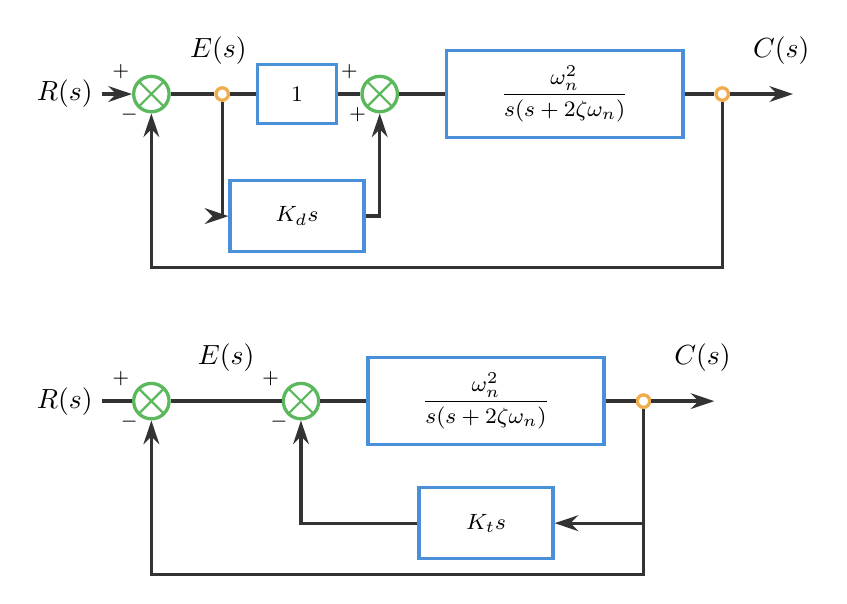
\begin{tikzpicture}[x=1cm, y=1cm]
  % PD structure
  \node (r1) at (0,0) {$R(s)$};
  \node[sum] (sum11) at (1.1,0) {};
  \node[tap] (tap11) at (2.0,0) {};
  \node at (1.95,0.55) {$E(s)$};
  \node[smallblock] (unit1) at (2.95,0) {$1$};
  \node[sum] (sum12) at (4.0,0) {};
  \node[plant] (plant1) at (6.35,0) {$\dfrac{\omega_n^2}{s(s+2\zeta\omega_n)}$};
  \node[tap] (tap12) at (8.35,0) {};
  \node at (9.1,0.55) {$C(s)$};
  \node[auxblock] (kd1) at (2.95,-1.55) {$K_d s$};

  \draw[signal] (r1) -- (sum11);
  \draw[signal] (sum11) -- (tap11) -- (unit1) -- (sum12) -- (plant1) -- (tap12) -- ++(0.9,0);
  \draw[signal] (tap11) |- (kd1);
  \draw[signal] (kd1) -| (sum12.south);
  \draw[signal] (tap12) |- ++(0,-2.2) -| (sum11.south);

  \node[sign] at ($(sum11.west)+(-0.14,0.28)$) {$+$};
  \node[sign] at ($(sum11.south)+(-0.28,-0.02)$) {$-$};
  \node[sign] at ($(sum12.west)+(-0.14,0.28)$) {$+$};
  \node[sign] at ($(sum12.south)+(-0.28,-0.02)$) {$+$};

  % Rate-feedback structure
  \node (r2) at (0,-3.9) {$R(s)$};
  \node[sum] (sum21) at (1.1,-3.9) {};
  \node at (2.05,-3.35) {$E(s)$};
  \node[sum] (sum22) at (3.0,-3.9) {};
  \node[plant] (plant2) at (5.35,-3.9) {$\dfrac{\omega_n^2}{s(s+2\zeta\omega_n)}$};
  \node[tap] (tap22) at (7.35,-3.9) {};
  \node at (8.1,-3.35) {$C(s)$};
  \node[auxblock] (kt2) at (5.35,-5.45) {$K_t s$};

  \draw[signal] (r2) -- (sum21) -- (sum22) -- (plant2) -- (tap22) -- ++(0.9,0);
  \draw[signal] (tap22) |- (kt2.east);
  \draw[signal] (kt2) -| (sum22.south);
  \draw[signal] (tap22) |- ++(0,-2.2) -| (sum21.south);

  \node[sign] at ($(sum21.west)+(-0.14,0.28)$) {$+$};
  \node[sign] at ($(sum21.south)+(-0.28,-0.02)$) {$-$};
  \node[sign] at ($(sum22.west)+(-0.14,0.28)$) {$+$};
  \node[sign] at ($(sum22.south)+(-0.28,-0.02)$) {$-$};
\end{tikzpicture}
\end{document}
